\documentclass[11pt]{article}
\usepackage{amsmath,amssymb,amsthm}
\usepackage[margin=1in]{geometry}
\usepackage{booktabs}
\usepackage{tikz}
\usepackage{hyperref}
\usepackage{xcolor}
\hypersetup{colorlinks=true, linkcolor=blue!50!black, urlcolor=blue!50!black}

\newcommand{\code}[1]{\texttt{#1}}

\title{Cauchy--Kovalevskaya, Riquier, and the\\ parametric data of ansatz 5}
\author{}
\date{July 7, 2026}

\begin{document}
\maketitle

\noindent
A companion note to \emph{A New Method of Solving PDEs}, expanding the
remark that ``Riquier's existence theorem gives a unique analytic solution
for any consistent choice of the parametric (free) data --- the rigorous
Cauchy--Kovalevskaya generalization.''  It records what the
principal/parametric split actually looks like --- the staircase picture ---
and works it out concretely for the hydrogen PDE under ansatz~5, where the
parametric data collapses to thirteen constants and Riquier's theorem
degenerates to ODE existence.

\section{The Cauchy--Kovalevskaya theorem}

The Cauchy--Kovalevskaya (CK) theorem is the fundamental
existence-and-uniqueness theorem for analytic PDEs.  Consider a system in
\emph{CK form} --- solved for the highest pure derivative in one
distinguished variable, say $t$:
\begin{equation*}
\frac{\partial^k u}{\partial t^k} = F(t, x, u, \ldots)
\end{equation*}
where $F$ is analytic in its arguments and the right-hand side involves
only derivatives of order $\le k$ having fewer than $k$ derivatives in
$t$.  If one prescribes \emph{analytic Cauchy data} --- the $k$ functions
$u, \partial_t u, \ldots, \partial_t^{k-1}u$ on the hypersurface $t=0$, as
analytic functions of $x$ --- then a \emph{unique analytic solution}
exists in a neighborhood of the hypersurface.

The proof is formal power series plus convergence: the equation determines
every Taylor coefficient of $u$ from the Cauchy data (each application of
$\partial_t^k$ is given by lower data), and the method of majorants shows
the series converges.  Cauchy proved the first-order case (1842);
Kovalevskaya gave the general formulation in her 1875
dissertation~\cite{kowalevsky}.

Two limitations matter here:
\begin{itemize}
\item \textbf{Only the ``solved'' (determined) form.}  CK says nothing
  about overdetermined systems --- several PDEs on one unknown, where
  cross-differentiation produces integrability conditions.
\item \textbf{Analytic category only.}  Lewy's example~\cite{lewy} shows
  existence can fail outright in the smooth category, and Kovalevskaya's
  heat-equation example shows the series can diverge when the equation is
  not in CK form.
\end{itemize}

\section{Riquier's generalization}

Riquier's theorem~\cite{riquier} extends CK to \emph{orthonomic (passive)
systems}.  Once an overdetermined system has been completed to passive
form --- all integrability conditions accounted for, which is exactly what
Rosenfeld--Gr\"obner or Thomas decomposition produces --- the derivatives
split, relative to the ranking, into:
\begin{itemize}
\item \textbf{principal} derivatives: those in the cone generated by the
  leaders (derivatives of the leading derivatives), determined by the
  equations; and
\item \textbf{parametric} derivatives: everything else.
\end{itemize}
Riquier: prescribe the parametric derivatives' values (analytic initial
data respecting the ranking) freely; there is then a unique analytic
solution.  The parametric derivatives of a regular differential chain
genuinely parameterize its solution set, and counting them (the
differential dimension / Hilbert--Kolchin polynomial~\cite{kolchin})
measures the size of the solution space.

\section{The staircase picture --- when is the parametric set finite?}

A natural first reaction is that CK data (a set of \emph{functions}) is
far more data than Riquier's parametric data (a set of
\emph{parameters}).  It is not: the two carry the same amount of data,
and the parametric set is finite only in a special case.

Identify each derivative $\partial_x^a\partial_t^b u$ with the lattice
point $(a,b)\in\mathbb{N}^2$.  A leader at $(a_0,b_0)$ claims as
principal the shifted quadrant $(a_0,b_0)+\mathbb{N}^2$.  The parametric
derivatives are the uncovered lattice points.  The complement of a union
of shifted quadrants is finite \emph{iff the leaders include a pure power
of every variable} --- a leader on each coordinate axis (the
monomial-ideal fact: $\mathbb{N}^n\setminus I$ is finite iff $I$ contains
some $x_i^{k_i}$ for every $i$).

\paragraph{Heat equation.}
Take $u_{xx}=u_t$, ranked so the leader is $u_{xx}$, at $(2,0)$:

\begin{center}
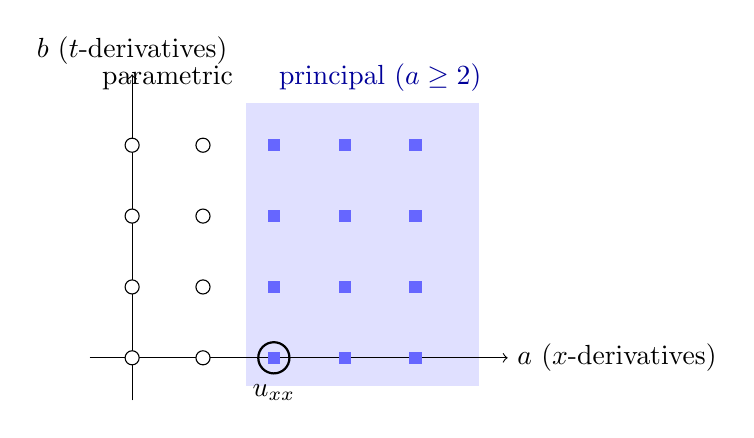
\begin{tikzpicture}[scale=0.9]
  \fill[blue!12] (1.6,-0.4) rectangle (4.9,3.6);
  \draw[->] (-0.6,0) -- (5.3,0) node[right] {$a$ ($x$-derivatives)};
  \draw[->] (0,-0.6) -- (0,4.0) node[above] {$b$ ($t$-derivatives)};
  \foreach \a in {2,3,4} \foreach \b in {0,1,2,3}
    \node[fill=blue!60, inner sep=2.2pt] at (\a,\b) {};
  \foreach \a in {0,1} \foreach \b in {0,1,2,3}
    \node[circle, draw, fill=white, inner sep=1.8pt] at (\a,\b) {};
  \draw[thick] (2,0) circle (0.22) node[below=6pt] {$u_{xx}$};
  \node[blue!60!black] at (3.5,3.95) {principal ($a\ge 2$)};
  \node at (0.5,3.95) {parametric};
\end{tikzpicture}
\end{center}

Nothing caps the $t$-axis, so the parametric set is the two infinite
columns $a\in\{0,1\}$.  Prescribing all Taylor coefficients in column
$a{=}0$ is prescribing the arbitrary analytic function $u(0,t)$; column
$a{=}1$ is $u_x(0,t)$.  One infinite strip $\leftrightarrow$ one free
\emph{function}.  This is exactly CK data for the equation read with $x$
as the evolution direction --- on a determined system, Riquier
specializes to CK, same data re-indexed.

\paragraph{Overdetermined case.}
Now a system whose leaders are $u_{xx}$ \emph{and} $u_{tt}$
(integrability conditions already satisfied):

\begin{center}
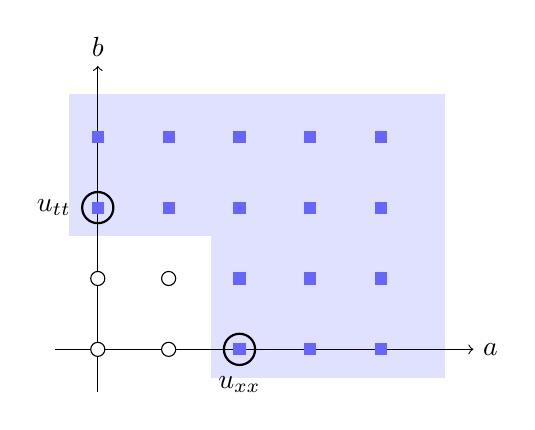
\begin{tikzpicture}[scale=0.9]
  \fill[blue!12] (1.6,-0.4) rectangle (4.9,3.6);
  \fill[blue!12] (-0.4,1.6) rectangle (4.9,3.6);
  \draw[->] (-0.6,0) -- (5.3,0) node[right] {$a$};
  \draw[->] (0,-0.6) -- (0,4.0) node[above] {$b$};
  \foreach \a in {2,3,4} \foreach \b in {0,1}
    \node[fill=blue!60, inner sep=2.2pt] at (\a,\b) {};
  \foreach \a in {0,1,2,3,4} \foreach \b in {2,3}
    \node[fill=blue!60, inner sep=2.2pt] at (\a,\b) {};
  \foreach \a in {0,1} \foreach \b in {0,1}
    \node[circle, draw, fill=white, inner sep=1.8pt] at (\a,\b) {};
  \draw[thick] (2,0) circle (0.22) node[below=6pt] {$u_{xx}$};
  \draw[thick] (0,2) circle (0.22) node[left=6pt] {$u_{tt}$};
\end{tikzpicture}
\end{center}

Every axis carries a leader; the parametric set is
$\{u, u_x, u_t, u_{xt}\}$ --- four constants.  The solution space is a
4-dimensional affine space: the differentially \emph{zero-dimensional},
ODE-like case, and the only situation where ``a finite set of
parameters'' is accurate.  A single PDE in ${\ge}\,2$ independent
variables can never achieve this --- one leader caps one quadrant,
leaving infinite strips.

Janet's decomposition~\cite{janet} makes the correspondence exact: the
parametric complement splits into disjoint cones (base point plus freedom
in the ``multiplicative'' directions), and each cone of dimension $d$
contributes one arbitrary analytic function of $d$ variables to the
initial data.  Counting parametric points of order $\le s$ gives the
\emph{Hilbert--Kolchin polynomial}: degree $n-1$ with leading coefficient
$k$ $\leftrightarrow$ ``$k$ arbitrary functions of $n-1$ variables'' (the
CK picture); eventually constant $\leftrightarrow$ finitely many
constants (zero-dimensional).  For overdetermined systems, Riquier's data
is genuinely \emph{smaller} than naive per-equation Cauchy data --- the
integrability conditions move derivatives into the principal cone --- and
is precisely the freedom the solution set actually has.

\section{Ansatz 5: the staircase ground down to a point}

Ansatz~5 (the second-order-ODE ansatz of \emph{A New Method of Solving
PDEs}; \code{finish\_prep(5)} in \code{helium.sage}) is the extreme case:
it caps every axis for every unknown, so the parametric set is finite
\emph{by design}.

The differential indeterminates over
$\mathbb{Q}\{x,y,z\}[r]/(r^2-x^2-y^2-z^2)$ are $\Psi$, $\Psi'$, $\Psi''$,
$v$, plus the 11 constants
$E, v_1,\ldots,v_4, a_0,a_1,b_0,b_1,c_0,c_1$.  The ansatz equations and
their leaders:

\begin{center}
\begin{tabular}{lll}
\toprule
equation & leader & order \\
\midrule
$v = v_1x+v_2y+v_3z+v_4r$ & $v$ & 0 \\
$(a_0{+}a_1v)\Psi'' + (b_0{+}b_1v)\Psi' + (c_0{+}c_1v)\Psi = 0$
  & $\Psi''$ & 0 \\
$\Psi_x=\Psi'v_x,\quad \Psi_y=\Psi'v_y,\quad \Psi_z=\Psi'v_z$
  & $\Psi_x,\Psi_y,\Psi_z$ & 1 \\
$\Psi'_x=\Psi''v_x,\quad \Psi'_y=\Psi''v_y,\quad \Psi'_z=\Psi''v_z$
  & $\Psi'_x,\Psi'_y,\Psi'_z$ & 1 \\
(constants) $\partial c=0$ & first derivatives & 1 \\
\bottomrule
\end{tabular}
\end{center}

Per-indeterminate staircases in $\mathbb{N}^3$
($\partial_x^a\partial_y^b\partial_z^c$):
\begin{itemize}
\item \textbf{$\Psi$}: leaders at $(1,0,0)$, $(0,1,0)$, $(0,0,1)$ --- a
  pure first derivative on every axis.  Parametric set: $\{\Psi\}$.  One
  constant.
\item \textbf{$\Psi'$}: identical.  Parametric set: $\{\Psi'\}$.  One
  constant.
\item \textbf{$\Psi''$, $v$}: leader at the origin --- solved outright
  ($\Psi''$ rationally from the ODE relation, $v$ explicitly).
  Parametric set: \emph{empty}.
\item \textbf{each constant}: only the order-0 value survives.  Eleven
  parameters --- but not free ones (\S\ref{sec:consistency}).
\end{itemize}

Where the raw Schr\"odinger equation alone (one leader in 3 variables)
leaves two infinite slabs --- Cauchy data of two arbitrary analytic
functions of two variables, dimension polynomial growing like $s^2$ ---
ansatz~5 grinds the staircase down until the Hilbert--Kolchin polynomial
is eventually constant.  Total parametric data: $\Psi(p_0)$,
$\Psi'(p_0)$, and the 11 constants --- thirteen numbers, modulo the two
homogenization scalings (\code{homogenize\_groups = (Avars, Vvars)} in
\code{helium.sage}), which are gauge.

\section{Where Riquier's theorem lands on ansatz 5}
\label{sec:consistency}

Riquier's ``unique analytic solution for any \emph{consistent} choice of
the parametric data'' plays out in two layers on ansatz~5:

\begin{enumerate}
\item \textbf{Consistency is where all the work lives.}  The chain-rule
  equations are automatically integrable (cross-derivatives agree because
  $v$ is explicit and $v_{xy}=v_{yx}$).  The genuine condition comes from
  reducing the Schr\"odinger PDE modulo the ansatz by Ritt
  reduction~\cite{ritt} (\code{differential\_prem} in \code{joca.sage}):
  the remainder must vanish identically, and its coefficients --- as a
  polynomial in $\Psi$, $\Psi'$ and the coordinates --- form a system of
  \emph{algebraic} equations in the 11 constants.  That polynomial system
  is exactly the input whose minimal primes \code{minprimes.sage}
  computes.  Consistency of the parametric data $=$ the constants lie on
  that variety.
\item \textbf{Existence then costs nothing.}  For each point of each
  prime component, Riquier hands a unique analytic solution per choice of
  the two remaining truly-free parameters $\Psi(p_0), \Psi'(p_0)$ ---
  which is just the classical fact that a second-order linear ODE has a
  2-dimensional solution space.  On this ansatz, Riquier degenerates all
  the way to ODE existence; no genuine PDE-analytic content remains.
\end{enumerate}

That is the shape of the whole program in staircase terms: the ansatz
converts ``solve a PDE'' (infinite-dimensional parametric data, degree-2
dimension polynomial) into ``find the variety where finite parametric
data is consistent'' (commutative algebra in 11 variables).  Every
hydrogen solution the ansatz can see corresponds to a point on one of the
minimal primes plus two ODE integration constants.

\begin{thebibliography}{9}

\bibitem{kowalevsky} S.~von Kowalevsky,
\emph{Zur Theorie der partiellen Differentialgleichungen},
J.\ Reine Angew.\ Math.\ \textbf{80} (1875), 1--32.

\bibitem{riquier} C.~Riquier,
\emph{Les syst\`emes d'\'equations aux d\'eriv\'ees partielles},
Gauthier-Villars, Paris, 1910.

\bibitem{janet} M.~Janet,
\emph{Le\c{c}ons sur les syst\`emes d'\'equations aux d\'eriv\'ees
partielles}, Gauthier-Villars, Paris, 1929.

\bibitem{ritt} J.~F.~Ritt,
\emph{Differential Algebra},
AMS Colloquium Publications \textbf{33}, American Mathematical Society,
1950.

\bibitem{lewy} H.~Lewy,
\emph{An example of a smooth linear partial differential equation without
solution}, Ann.\ of Math.\ \textbf{66} (1957), 155--158.

\bibitem{kolchin} E.~R.~Kolchin,
\emph{Differential Algebra and Algebraic Groups},
Academic Press, New York, 1973.

\end{thebibliography}

\bigskip
\noindent{\small /Claude (Fable 5)}

\end{document}
